\begin{landscape}
	

\begin{figure} % "[t!]" placement specifier just for this example
	\centering 
	

	\begin{subfigure}{0.37\textwidth}
		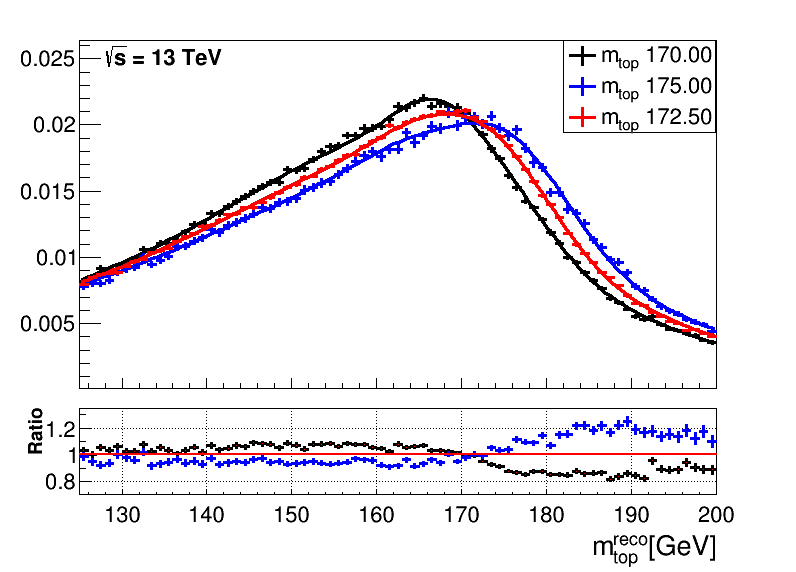
\includegraphics[width=\linewidth]{Pics/PlotCombi/mtop_mtop.png}
		\caption{$m_{\rm top}^{\rm reco}$ vs $m_{\rm top}$} \label{fig:mtopmtop}
	\end{subfigure}
	\hspace*{0.25cm}
	\begin{subfigure}{0.37\textwidth}
	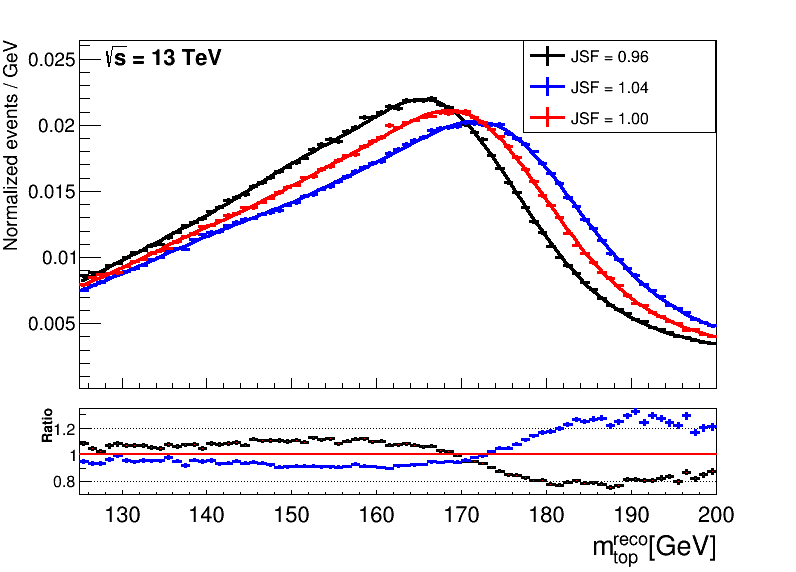
\includegraphics[width=\linewidth]{Pics/PlotCombi/mtop_JSF.png}
	\caption{$m_{\rm top}^{\rm reco}$ vs JSF} \label{fig:mtopJSF}
	\end{subfigure}
	\hspace*{0.25cm}
	\begin{subfigure}{0.37\textwidth}
	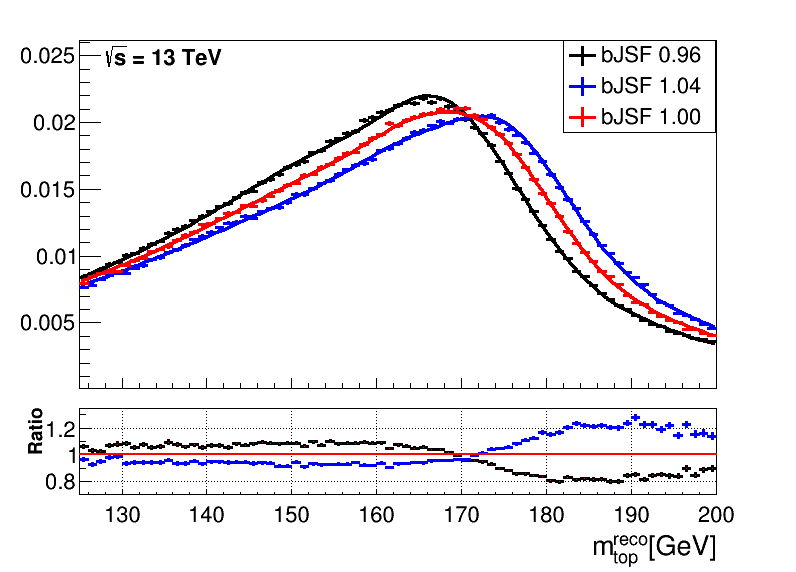
\includegraphics[width=\linewidth]{Pics/PlotCombi/mtop_bJSF.png}
	\caption{$m_{\rm top}^{\rm reco}$ vs bJSF} \label{fig:mtopbJSF}
	\end{subfigure}
	\begin{subfigure}{0.37\textwidth}
	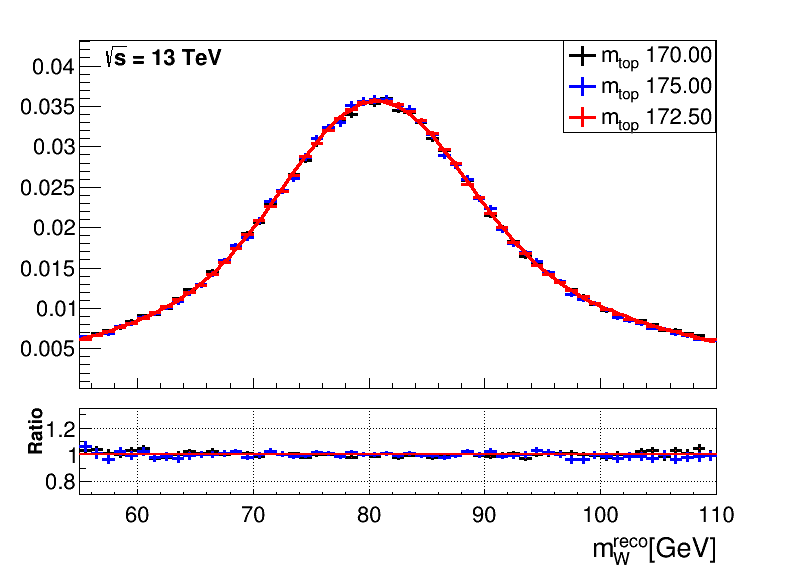
\includegraphics[width=\linewidth]{Pics/PlotCombi/mw_mtop.png}
	\caption{$m_{\rm W}^{\rm reco}$ vs $m_{\rm top}$} \label{fig:mwmtop}
	\end{subfigure}
	\hspace*{0.25cm}
	\begin{subfigure}{0.37\textwidth}
	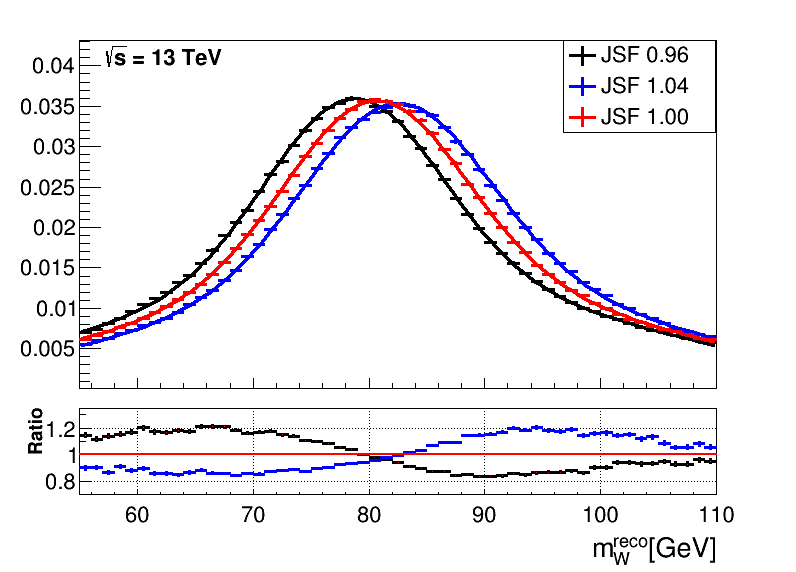
\includegraphics[width=\linewidth]{Pics/PlotCombi/mw_JSF.png}
	\caption{$m_{\rm W}^{\rm reco}$ vs JSF} \label{fig:mwJSF}
	\end{subfigure}
	\hspace*{0.25cm}
	\begin{subfigure}{0.37\textwidth}
	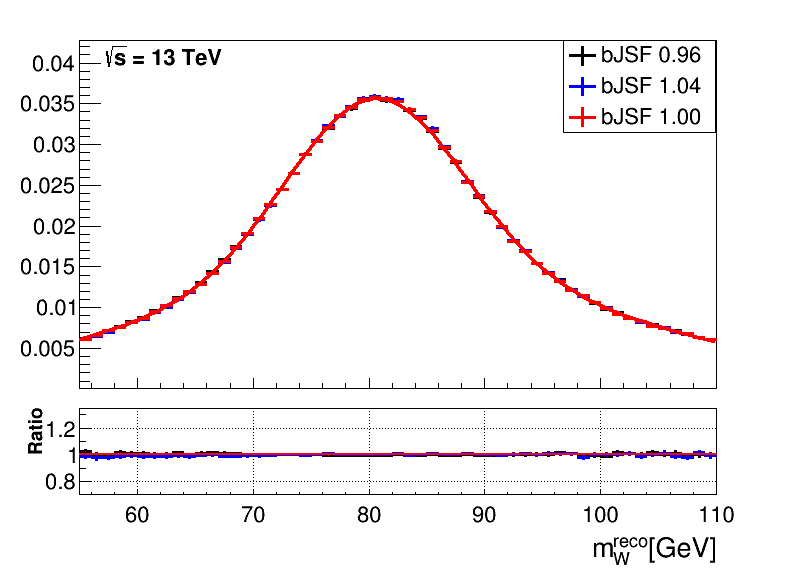
\includegraphics[width=\linewidth]{Pics/PlotCombi/mw_bJSF.png}
	\caption{$m_{\rm W}^{\rm reco}$ vs bJSF} \label{fig:mwbJSF}
	\end{subfigure}
	\begin{subfigure}{0.37\textwidth}
	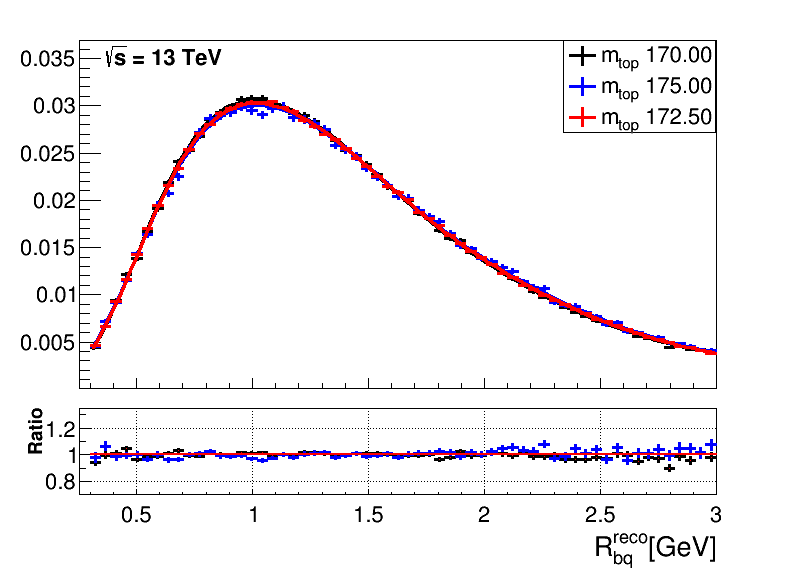
\includegraphics[width=\linewidth]{Pics/PlotCombi/rbq_mtop.png}
	\caption{$R_{\rm bq}^{\rm reco}$ vs $m_{\rm top}$} \label{fig:Rbqmtop}
\end{subfigure}
\hspace*{0.25cm}
\begin{subfigure}{0.37\textwidth}
	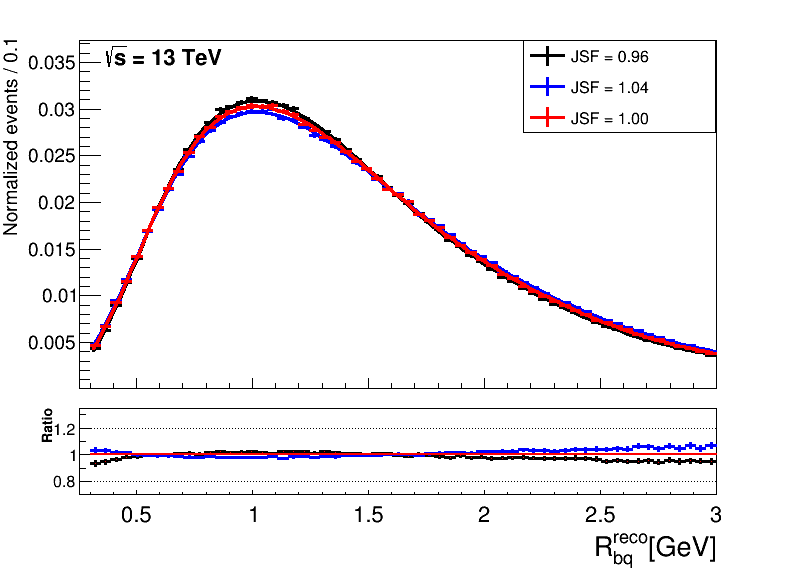
\includegraphics[width=\linewidth]{Pics/PlotCombi/rbq_JSF.png}
	\caption{$R_{\rm bq}^{\rm reco}$ vs JSF} \label{fig:RbqJSF}
\end{subfigure}
\hspace*{0.25cm}
\begin{subfigure}{0.37\textwidth}
	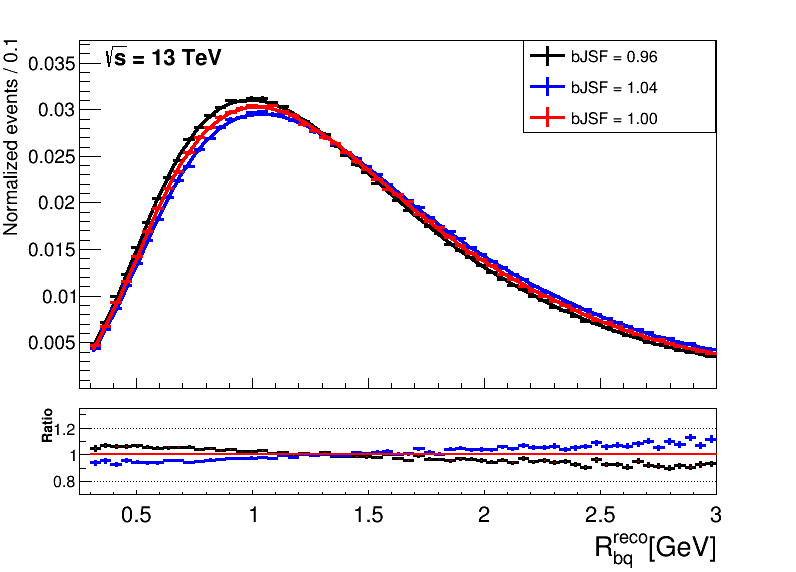
\includegraphics[width=\linewidth]{Pics/PlotCombi/rbq_bJSF.png}
	\caption{$R_{\rm bq}^{\rm reco}$ vs bJSF} \label{fig:RbqbJSF}
\end{subfigure}
	\caption{Comparison of signal $t\bar{t}$ templates for different simulated top-quark masses and scale factors. For each of the three observables, ($m_{\rm top}^{\rm reco}$, $m_{\rm W}^{\rm reco}$ and $R_{\rm bq}^{\rm reco}$) the sensitivities are displayed, by overlaying the nominal (red) sample with samples for different JSF, bJSF and $m_{\rm top}$ . The unvaried quantity is kept to the nominal value. }
\label{fig:Comparison}	
\end{figure}
\end{landscape}